\section{Expanded experiment on 160 Slakh2100-redux tracks}
\label{sec:slakh160}

\subsection{Data and training}
The follow-up samples tracks with seed 5305 from the official Slakh2100-redux training, validation and test partitions \cite{slakhredux}. The pinned download manifest identifies all tracks and source files. An assertion checks that identical full-track MIDI hashes do not cross partitions. Mono audio is resampled to 16\,kHz and split into complete five-second clips. Each clip has an original mix, a two-family absence mix and a mix with controlled starts or stops. The 120 training, 20 validation and 20 test tracks yield 17,670, 2,985 and 3,051 examples including all variants. The test partition contains 1,017 original clips.

Mean, max and attention pooling use the same encoder and clip-label loss. Each model was trained once with seed 5305. Checkpoints were selected by validation clip macro balanced accuracy. Frame thresholds were calibrated on the validation MIDI references and fixed for test evaluation. Event scoring uses a 0.5\,s tolerance at both endpoints with clip-edge censoring, as in the BabySlakh follow-up.

\subsection{Recognition and localisation results}
\begin{table}[htbp]
\centering
\small
\caption{Results on the 160-track subset, one run per pooling method. Frame BA is macro balanced accuracy. Pooled results combine the original, absence and transition variants.}
\label{tab:slakh160}
\begin{tabular}{lrrrrr}
\toprule
Pooling & Val.\ clip BA & Test clip BA & Original frame BA & Pooled frame BA & Pooled event F1\\
\midrule
Mean & 0.740 & 0.740 & 0.689 & 0.682 & 0.228\\
Max & \textbf{0.814} & \textbf{0.819} & 0.635 & 0.652 & 0.108\\
Attention & 0.790 & 0.784 & \textbf{0.707} & \textbf{0.699} & \textbf{0.260}\\
\bottomrule
\end{tabular}
\end{table}

Max pooling led clip-level validation and test recognition. Attention scored highest on frame-level test localisation for original mixes and for the pooled variants (Table~\ref{tab:slakh160}). On absence and transition mixes, its frame BA was 0.703 for each after rounding. The pooled always-active baseline achieved frame BA of 0.500. Attention's pooled event F1 of 0.260 shows that locating complete intervals remains difficult, even when many individual bins are classified correctly.

\clearpage
\subsection{Validation examples shown in the demonstration}
\begin{figure}[H]
\centering
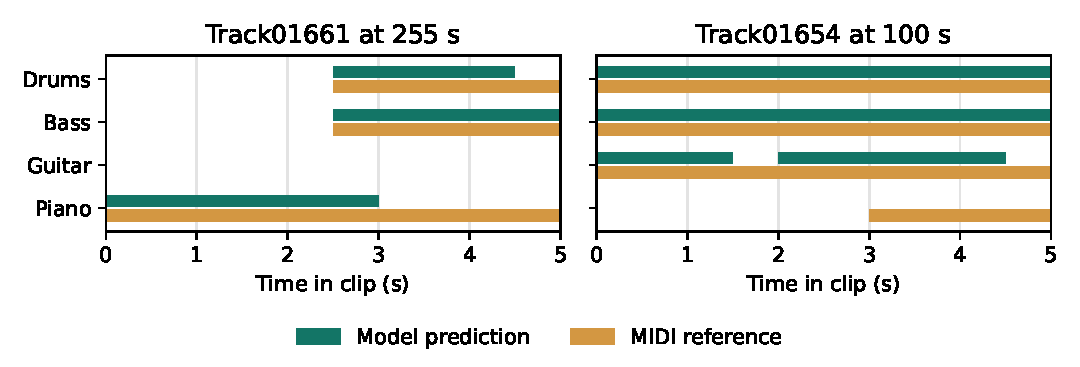
\includegraphics[width=\linewidth]{figures/slakh160_demo.pdf}
\caption{Attention checkpoint outputs and MIDI reference activity for two selected validation excerpts. Times are relative to each five-second clip. The excerpts illustrate a matching bass onset and a missed piano interval.}
\label{fig:slakh160-demo}
\end{figure}

In \code{Track01661}, the predicted and reference bass intervals begin at 2.5\,s and extend to the clip boundary. In \code{Track01654}, the MIDI reference shows piano activity from 3.0 to 5.0\,s and the model produces no piano interval (Figure~\ref{fig:slakh160-demo}). The video shows inference on the WAV excerpts. These examples are selected from the validation set and the aggregate scores come from the held-out test partition.

The BabySlakh and 160-track experiments use different held-out tracks. Comparing 0.629 with 0.699 describes results on those two evaluations. A shared test set and matched training protocol would be needed to estimate the effect of increasing the training set. The single-seed follow-up also leaves between-run variation unmeasured.
